\setmainfont{Noteworthy}

\begin{frame}
\frametitle{Connectivity in Graphs}
\begin{itemize}
    \item Today, we are talking about connectivity in graphs.
    \item Following are examples of two connected graphs.
\end{itemize}
\vspace*{10pt}
\begin{columns}
    \begin{column}{0.5\textwidth}
        \centering
        \textbf{Graph (A)}
        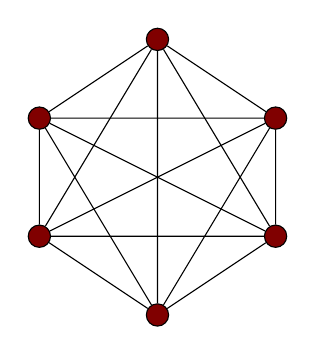
\begin{tikzpicture}
            \node[circle, color=black, fill={rgb,255:red,128; green,0; blue,0}, draw, inner sep=0.1cm] (a1) at (0, 1.5) {};
            \node[circle, color=black, fill={rgb,255:red,128; green,0; blue,0}, draw, inner sep=0.1cm] (a2) at (1.5, 2.5) {};
            \node[circle, color=black, fill={rgb,255:red,128; green,0; blue,0}, draw, inner sep=0.1cm] (a3) at (3, 1.5) {};
            \node[circle, color=black, fill={rgb,255:red,128; green,0; blue,0}, draw, inner sep=0.1cm] (a4) at (3, 0) {};
            \node[circle, color=black, fill={rgb,255:red,128; green,0; blue,0}, draw, inner sep=0.1cm] (a5) at (1.5, -1) {};
            \node[circle, color=black, fill={rgb,255:red,128; green,0; blue,0}, draw, inner sep=0.1cm] (a6) at (0, 0) {};

            \draw (a1) -- (a2) -- (a3) -- (a4) -- (a5) -- (a6) -- (a1);
            \draw (a6) -- (a3) -- (a1) -- (a4);
            \draw (a6) -- (a4) -- (a2);
            \draw (a6) -- (a2) -- (a5) -- (a1);
            \draw (a5) -- (a3);
        \end{tikzpicture}
    \end{column}
    \begin{column}{0.5\textwidth}
        \centering
        \textbf{Graph (B)}
        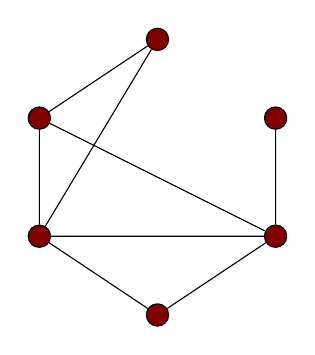
\begin{tikzpicture}
            \node[circle, color=black, fill={rgb,255:red,128; green,0; blue,0}, draw, inner sep=0.1cm] (b1) at (0, 1.5) {};
            \node[circle, color=black, fill={rgb,255:red,128; green,0; blue,0}, draw, inner sep=0.1cm] (b2) at (1.5, 2.5) {};
            \node[circle, color=black, fill={rgb,255:red,128; green,0; blue,0}, draw, inner sep=0.1cm] (b3) at (3, 1.5) {};
            \node[circle, color=black, fill={rgb,255:red,128; green,0; blue,0}, draw, inner sep=0.1cm] (b4) at (3, 0) {};
            \node[circle, color=black, fill={rgb,255:red,128; green,0; blue,0}, draw, inner sep=0.1cm] (b5) at (1.5, -1) {};
            \node[circle, color=black, fill={rgb,255:red,128; green,0; blue,0}, draw, inner sep=0.1cm] (b6) at (0, 0) {};

            \draw (b2) -- (b1) -- (b6) -- (b5) -- (b4) -- (b3);
            \draw (b2) -- (b6) -- (b4) -- (b1);
        \end{tikzpicture}
    \end{column}
\end{columns}
\vspace*{10pt}
\centering
\textit{Although both of these graphs are connected, intuitively they have different levels of connectivity.}
\end{frame}


\begin{frame}
    \frametitle{Articulation point in graph \( G \)}
    \textbf{Definition:} In a connected component \( G \), \( \exists \) a vertex that if removed,disconnects increases the number of connected components of the remaining graph. 
    \newline
    \textbf{Example:} Graph(B) in the last slide.
    \vspace{10pt} % Adds space before the graph
    
    \begin{minipage}{0.50\textwidth} % Reduced width for graph
        \begin{flushleft} % Aligns the graph to the left
            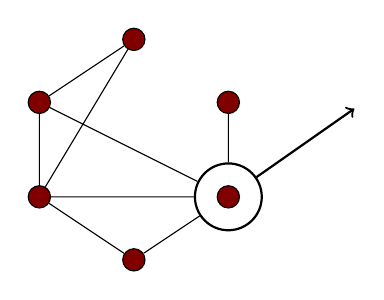
\begin{tikzpicture}[scale=0.8] % Keep same scale
                % Define nodes
               \node[circle, fill={rgb,255:red,128; green,0; blue,0}, draw, inner sep=0.1cm] (b1) at (0, 1.5) {};
                \node[circle, fill={rgb,255:red,128; green,0; blue,0}, draw, inner sep=0.1cm] (b2) at (1.5, 2.5) {};
                \node[circle,fill={rgb,255:red,128; green,0; blue,0}, draw, inner sep=0.1cm] (b3) at (3, 1.5) {};
                \node[circle, fill={rgb,255:red,128; green,0; blue,0}, draw, inner sep=0.1cm] (b4) at (3, 0) {};
                \node[circle, color=black, draw, inner sep=0.3cm, thick] (b4) at (3, 0) {}; % Larger, transparent node
                \node[circle, fill={rgb,255:red,128; green,0; blue,0}, draw, inner sep=0.1cm] (b5) at (1.5, -1) {};
                \node[circle, fill={rgb,255:red,128; green,0; blue,0}, draw, inner sep=0.1cm] (b6) at (0, 0) {};

                % Draw edges
                \draw (b2) -- (b1) -- (b6) -- (b5) -- (b4) -- (b3);
                \draw (b2) -- (b6) -- (b4) -- (b1);
                 \draw[->, thick] (b4) --++ (2, 1.4);
            \end{tikzpicture}
        \end{flushleft}
    \end{minipage}%
    \hspace{-40pt} % Move text further left
     \begin{minipage}{0.47\textwidth} % Increased width for text
        {\large \textbf{Note:}} If this vertex is removed, the graph will become disconnected.  
        \newline
        {\large Hence, it is an \textbf{Articulation Point} of Graph(B).}
    \end{minipage}

    \vspace{10pt} % Space before the P.S. note
    \begin{flushleft}
        \textbf{P.S.} There is no articulation point in Graph(A) because removing any vertex from it would not disconnect the graph.
    \end{flushleft}

\end{frame}


\begin{frame}
    \frametitle{Continuation}
    \large\textbf{For another Graph \( G \) below:}
    \vspace{5pt} % Reduced space before the graph

    \begin{minipage}{0.55\textwidth} % Graph on the left, slightly wider
        \begin{flushleft} 
            \begin{tikzpicture}[scale=1.3] % Increased scale for a larger graph
                % Define vertices with labels
                \node[circle, fill=maroon, draw, inner sep=0.12cm, label=above:\textbf{A}] (A) at (0, 2) {};
                \node[circle, fill=maroon, draw, inner sep=0.12cm, label=left:\textbf{B}] (B) at (-1.5, 1) {};
                \node[circle, fill=maroon, draw, inner sep=0.12cm, label=right:\textbf{C}] (C) at (1.5, 1) {};
                \node[circle, fill=maroon, draw, inner sep=0.12cm, label={[yshift=-6pt]below:\textbf{D}}] (D) at (0, 0) {};
                 \node[circle, color =black, draw, inner sep=0.30cm] (D) at (0, 0) {};% Marking D as articulation point
                \node[circle, fill=maroon, draw, inner sep=0.12cm, label=left:\textbf{E}] (E) at (-1.5, -1) {};
                \node[circle, fill=maroon, draw, inner sep=0.12cm, label=right:\textbf{F}] (F) at (1.5, -1) {};
                \draw (A) -- (B) -- (D) -- (E);
                \draw (A) -- (C) -- (D) -- (F);
                
            
            \end{tikzpicture}
        \end{flushleft}
    \end{minipage}%
    \hspace{-30pt} % Move text closer to the graph
    \begin{minipage}{0.45\textwidth} % Text on the right
        {\large \textbf{Vertex D is an articulation point. Removing it will disconnect the graph.}}
    \end{minipage}

    \vspace{10pt} % Space before bullet points
    \begin{itemize}
        \item Removing vertex \( D \) causes the graph to become disconnected, making it an articulation point.
        \item Other vertices are not articulation points because their removal does not disconnect the graph.
    \end{itemize}

\end{frame}







\begin{frame}
    \frametitle{Real World Example}
    \large\textbf{Consider critical infrastructure transmission networks of electricity containing single points of failure. These bottlenecks can disrupt entire systems when compromised.}
    
    \vspace*{15pt}
    \centering
    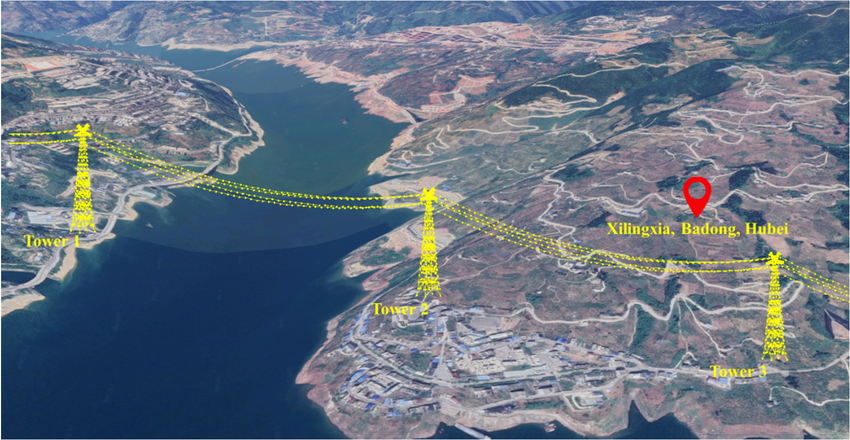
\includegraphics[width=0.6\textwidth]{figures/general/transmission-network.png}
    \vspace*{5pt}
    
    \textbf{Electrical Grid Vulnerability} \\
    \small A single transmission tower acting as bridge node between regional networks
\end{frame}

\begin{frame}
    \frametitle{Real World Example}
    \large\textbf{Bottlenecks create systemic risk - their failure partitions networks into disconnected components, halting flow and communication.}
    
    \vspace*{15pt}
    \centering
    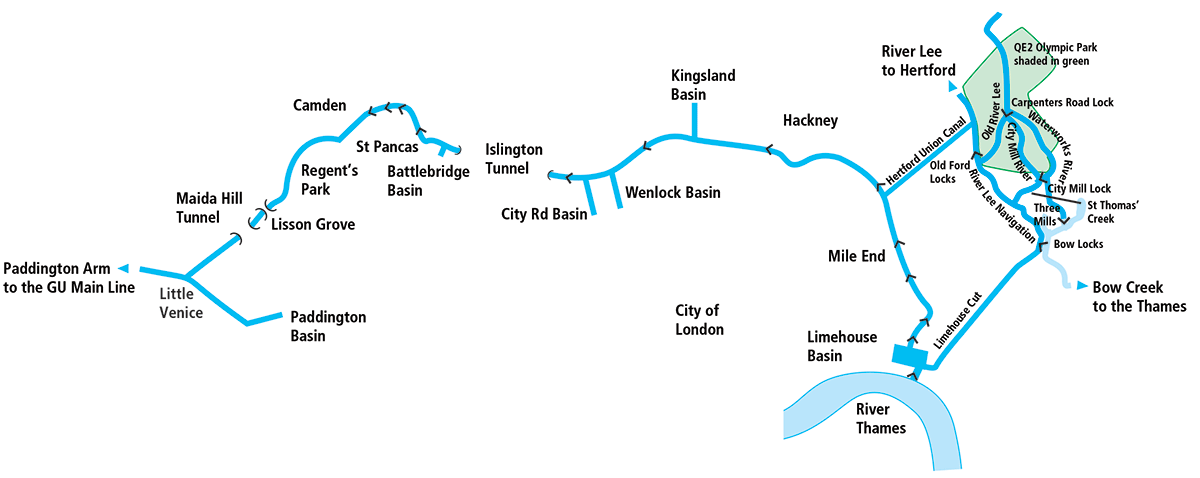
\includegraphics[width=0.6\textwidth]{figures/general/canal-network.png}
    \vspace*{5pt}
    
    \textbf{Waterway Chokepoint} \\
    \small Critical canal section enabling continental shipping routes
\end{frame}


\begin{frame}
    \frametitle{Observation}

    \begin{minipage}{0.50\textwidth} % Graph on the left
        \begin{flushleft}
            \begin{tikzpicture}
                % Define main node (shifted slightly right)
                \node[draw, circle, fill=maroon, inner sep=2.5pt] (N) at (1, 0) {};

                % Define subgraphs with cloud shapes
                \node[draw, cloud, cloud puffs=10, minimum width=2.5cm, minimum height=1.5cm] (T1) at (-0.5, 2) {\Large \( T_1 \)};
                \node[draw, cloud, cloud puffs=8, minimum width=1.8cm, minimum height=1cm] (T2) at (2.2, -1.6) {\normalsize \( T_2 \)};

                % Draw edges
                \draw (T1) -- (N) -- (T2);

                % Arrow from N to the explanation text
                \draw[->, thick] (N) --++ (2, 1.0);
            \end{tikzpicture}
        \end{flushleft}
    \end{minipage}%
    \hspace{-30pt} % Move text closer to the graph
    \begin{minipage}{0.50\textwidth} % Explanation on the right
        This is an \textbf{Articulation Point} as no edge connects subgraph \( T_1 \) to subgraph \( T_2 \) (or vice versa). \\
    \end{minipage}

\end{frame}

\begin{frame}
    \frametitle{In Computer Terminology}

    \begin{minipage}{0.42\textwidth} % Left side for text (slightly wider)
        \textbf{This is the only point connecting the two subgraphs \( T_1 \) and \( T_2 \).} \\
        If you need to go from \( T_1 \) to \( T_2 \), you must pass through this point.
    \end{minipage}%
    \hspace{5pt} % Reduced space between text and graph
    \begin{minipage}{0.53\textwidth} % Right side for the graph
        \begin{center}
            \begin{tikzpicture}
                % Define main node (shifted slightly right)
                \node[draw, circle, fill=maroon, inner sep=2.5pt] (N) at (1, 0) {};

                % Define subgraphs with cloud shapes
                \node[draw, cloud, cloud puffs=10, minimum width=2.5cm, minimum height=1.5cm] (T1) at (-0.5, 2) {\Large \( T_1 \)};
                \node[draw, cloud, cloud puffs=8, minimum width=1.8cm, minimum height=1cm] (T2) at (2.2, -1.6) {\normalsize \( T_2 \)};

                % Draw edges
                \draw (T1) -- (N) -- (T2);

                % Labels for visited and going to visit
                \node[right=1.3cm] at (T1) {\textbf{Visited}};
                \node[below=0.4cm] at (T2) {\textbf{Going to Visit}};

                % Arrow from node N to the left text
                \draw[->, thick] (N) --++ (-2.8, 0);
            \end{tikzpicture}
        \end{center}
    \end{minipage}
    {\fontsize{13}{16}\selectfont \textbf{{We will use a modified version of DFS.}}}
\end{frame}







\begin{frame}
    \frametitle{Informal Definition}

    \begin{center}
        \textbf{\textbf{\underline{Informally}}}, an edge from descendants to ancestors means it is not an articulation point.
    \end{center}

    \vspace{10pt} % Space between the text and the graph

    \begin{center} % Center the graph
        \begin{tikzpicture}
            % Define main node (shifted slightly right)
            \node[draw, circle, fill=maroon, inner sep=2.5pt] (N) at (1, 0) {};

            % Define subgraphs with cloud shapes
            \node[draw, cloud, cloud puffs=10, minimum width=2.5cm, minimum height=1.5cm] (T1) at (-0.5, 2) {\Large \( T_1 \)};
            \node[draw, cloud, cloud puffs=8, minimum width=1.8cm, minimum height=1cm] (T2) at (2.2, -1.6) {\normalsize \( T_2 \)};

            % Draw edges
            \draw (T1) -- (N) -- (T2);
            \draw[->, thick] (N) --++ (-0.8, 0);

            % Add curved edge with arrow from T2 to T1
            \draw[bend right=25, thick, ->] (T2) to (T1);

            % Labels for Ancestors and Descendants
            \node[right=1.3cm] at (T1) {\textbf{Ancestors}};
            \node[below=0.4cm] at (T2) {\textbf{Descendants}};

            % Add label to the left of node N
            \node[left=0.8cm] at (N) {\textbf{Not an articulation point}};
        \end{tikzpicture}
    \end{center}

\end{frame}

\begin{frame}
    \frametitle{Checks}

    \begin{enumerate}
        \item Root is an \underline{articulation point} if it has multiple ( > 1 ) children
        \item For non-root vertices: Check if any child's low $\geq$ discovery time of current node
    \end{enumerate}

    \vspace{10pt} % Space before the graphs

    \begin{center}
        \begin{tikzpicture}[scale=1.5]
            % Rule 0 Graph
            \begin{scope}
                \node[draw, circle, fill=maroon, inner sep=2pt, label=above:A] (A) at (0,1) {};
                \node[draw, circle, inner sep=5pt] (A_outer) at (0,1) {}; % Outer circle
                
                \node[draw, circle, fill=maroon, inner sep=2pt, label=left:B] (B) at (-0.87, 0.5) {};
                \node[draw, circle, fill=maroon, inner sep=2pt, label=left:C] (C) at (-0.87, -0.5) {};
                
                % Labels
                \node[right=0.8cm] at (A) {\scriptsize \textbf{Can't be } \\ \textbf{Articulation Point (if root)}};
                \node[right=0.8cm] at (B) {\scriptsize \textbf{Articulation Point}};

                % Graph Edges
                \draw (A) -- (B);
                \draw (B) -- (C);
            \end{scope}
            \node at (0.0, -0.9) {\textbf{Rule 0}};

            % Rule 1 Graph (Shifted to Right)
            \begin{scope}[xshift=4cm]
                \node[draw, circle, fill=maroon, inner sep=2pt, label=above:A] (A1) at (0,1) {};
                \node[draw, circle, inner sep=5pt] (A_outer1) at (0,1) {}; % Outer circle
                
                \node[draw, circle, fill=maroon, inner sep=2pt, label=left:B] (B1) at (-0.87, 0.5) {};
                \node[draw, circle, fill=maroon, inner sep=2pt, label=left:C] (C1) at (-0.87, -0.5) {};
                \node[draw, circle, fill=maroon, inner sep=2pt, label=right:D] (D1) at (0.87, 0.5) {};
                \node[draw, circle, fill=maroon, inner sep=2pt, label=right:E] (E1) at (0.87, -0.5) {}; 

                % Labels
                \node[above=0.5cm] at (A1) {\scriptsize \textbf{Root and Articulation Point}};

                % Graph Edges
                \draw (A1) -- (B1);
                \draw (B1) -- (C1);
                \draw (A1) -- (D1);
                \draw (D1) -- (E1);
            \end{scope}
            \node at (4.0, -0.9) {\textbf{Rule 1}};
        \end{tikzpicture}
    \end{center}
    \vspace{5pt} % Space before the added line
    \centering \textbf{Children means unvisited neighbors}
\end{frame}


\begin{frame}
    \frametitle{Example \# 01}

    \vspace*{10pt}
 \textbf{Let a Graph } \( G \):
    \newline
    \newline
     \textbf{Algorithm will start from (e)}

    \vspace{10pt} % Space before the graph

    \begin{center}
        \begin{tikzpicture}[scale=2] % Increased scale
            % Nodes filled with maroon
            \node[draw, circle, fill=maroon, inner sep=2pt] (a) at (1,2) {};
            \node[draw, circle, fill=maroon, inner sep=2pt] (b) at (0,1.5) {};
            \node[draw, circle, fill=maroon, inner sep=2pt] (c) at (0,1) {};
            \node[draw, circle, fill=maroon, inner sep=2pt] (d) at (0,0) {};
            \node[draw, circle, fill=maroon, inner sep=2pt] (e) at (2,1) {};
            \node[draw, circle, fill=maroon, inner sep=2pt] (f) at (2,0) {};
            \node[draw, circle, fill=maroon, inner sep=2pt] (g) at (2,-0.5) {}; % g below f

            % Labels outside the nodes (no fill color)
            \node[right=3pt] at (a) {\textbf{a}};
            \node[left=3pt] at (b) {\textbf{b}};
            \node[left=3pt] at (c) {\textbf{c}};
            \node[left=3pt] at (d) {\textbf{d}};
            \node[right=3pt] at (e) {\textbf{e}};
            \node[right=3pt] at (f) {\textbf{f}};
            \node[right=3pt] at (g) {\textbf{g}};

            % Edges
            \draw (a) -- (b);
            \draw (b) -- (c);
            \draw (c) -- (d);
            \draw (c) -- (e);
            \draw (d) -- (f);
            \draw (e) -- (f);
            \draw (f) -- (g); % f connected to g only
        \end{tikzpicture}
        
        % Right-side text
        \hspace{3cm} % Adjusts spacing to move text to the right
       
    \end{center}

\end{frame}


\begin{frame}
    \frametitle{Example \# 01 - Continue}
    \begin{center}
        \href{https://drive.google.com/file/d/1qEE1As0QusE928N4wITiYJYmUcZanK3L/view?usp=sharing}{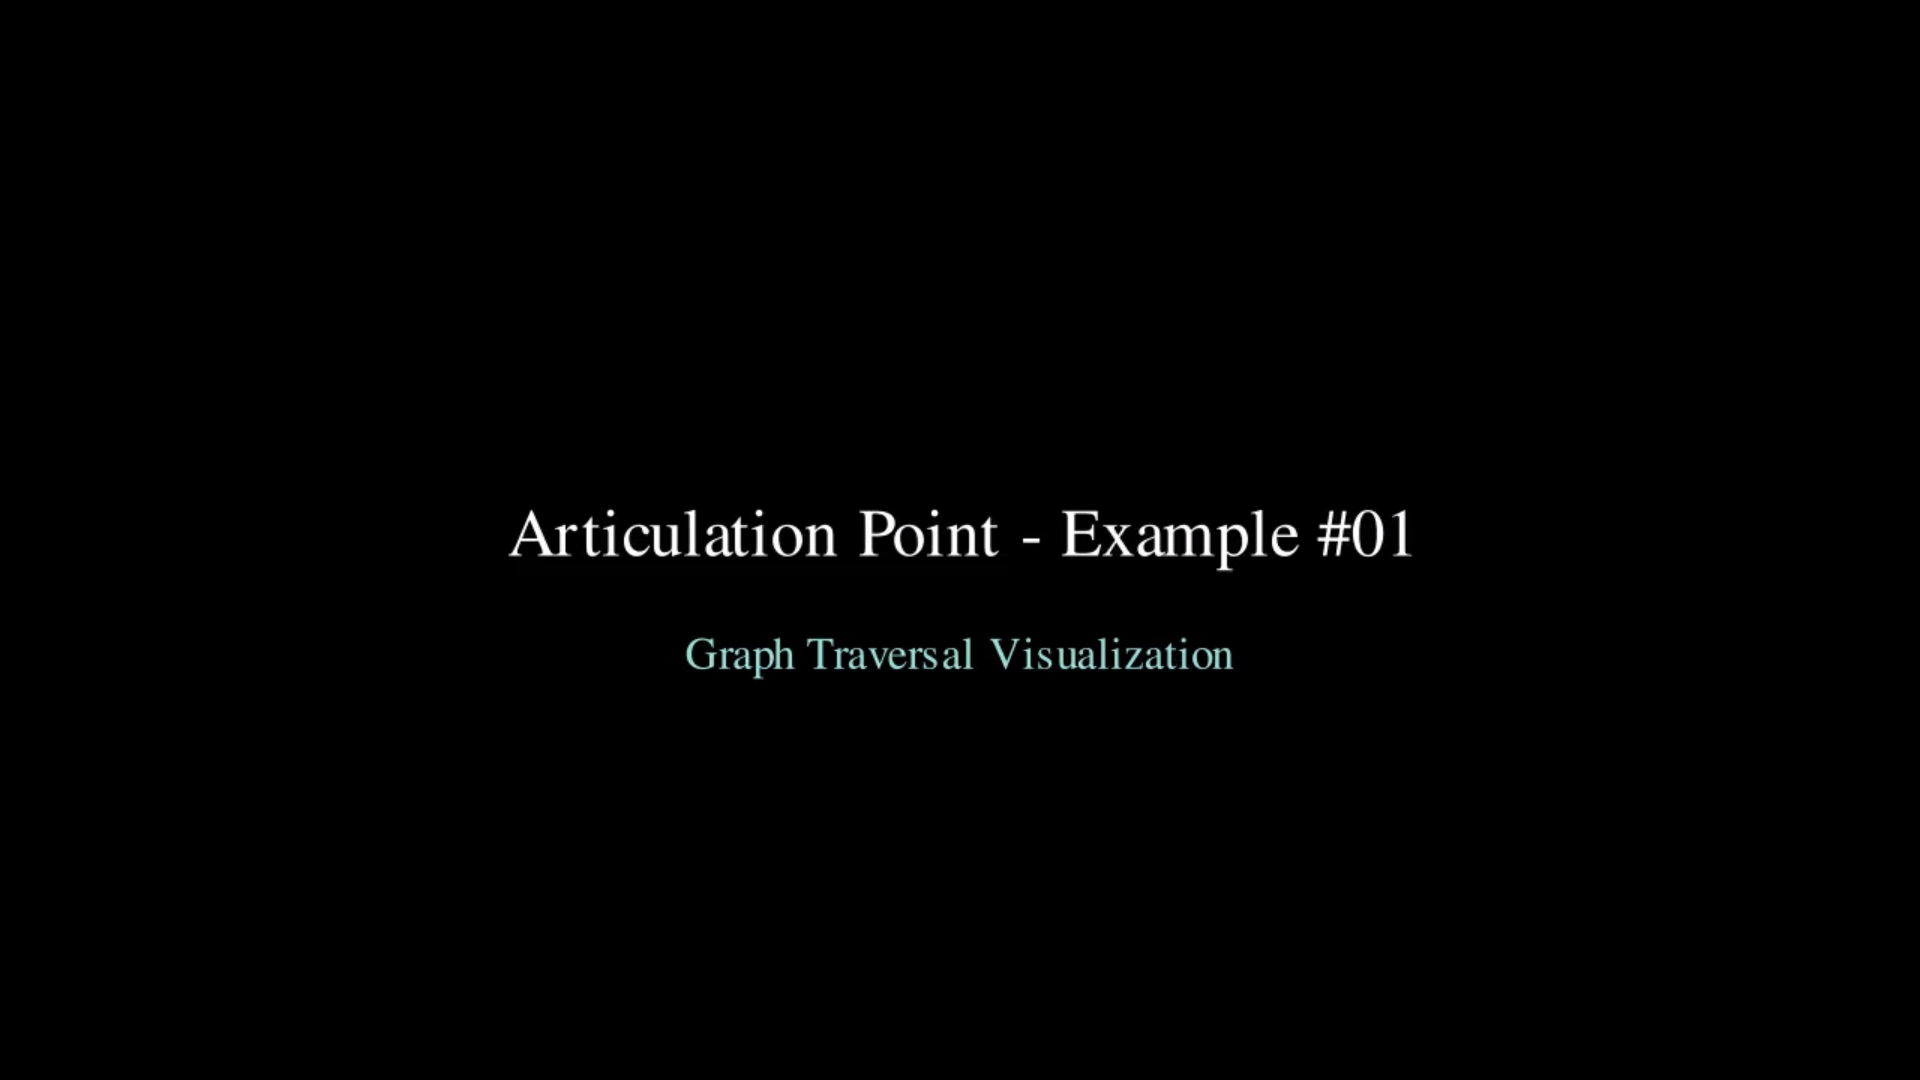
\includegraphics[width=\linewidth]{figures/general/exm01.png}}
    \end{center}
\end{frame}

\begin{frame}
    \frametitle{Example \# 01 - DFS Graph traversal}
    \begin{center}
        \href{https://drive.google.com/file/d/1h2zJHoirxqV9HhY3J9XQs5IgGjNX7waE/view?usp=sharing}{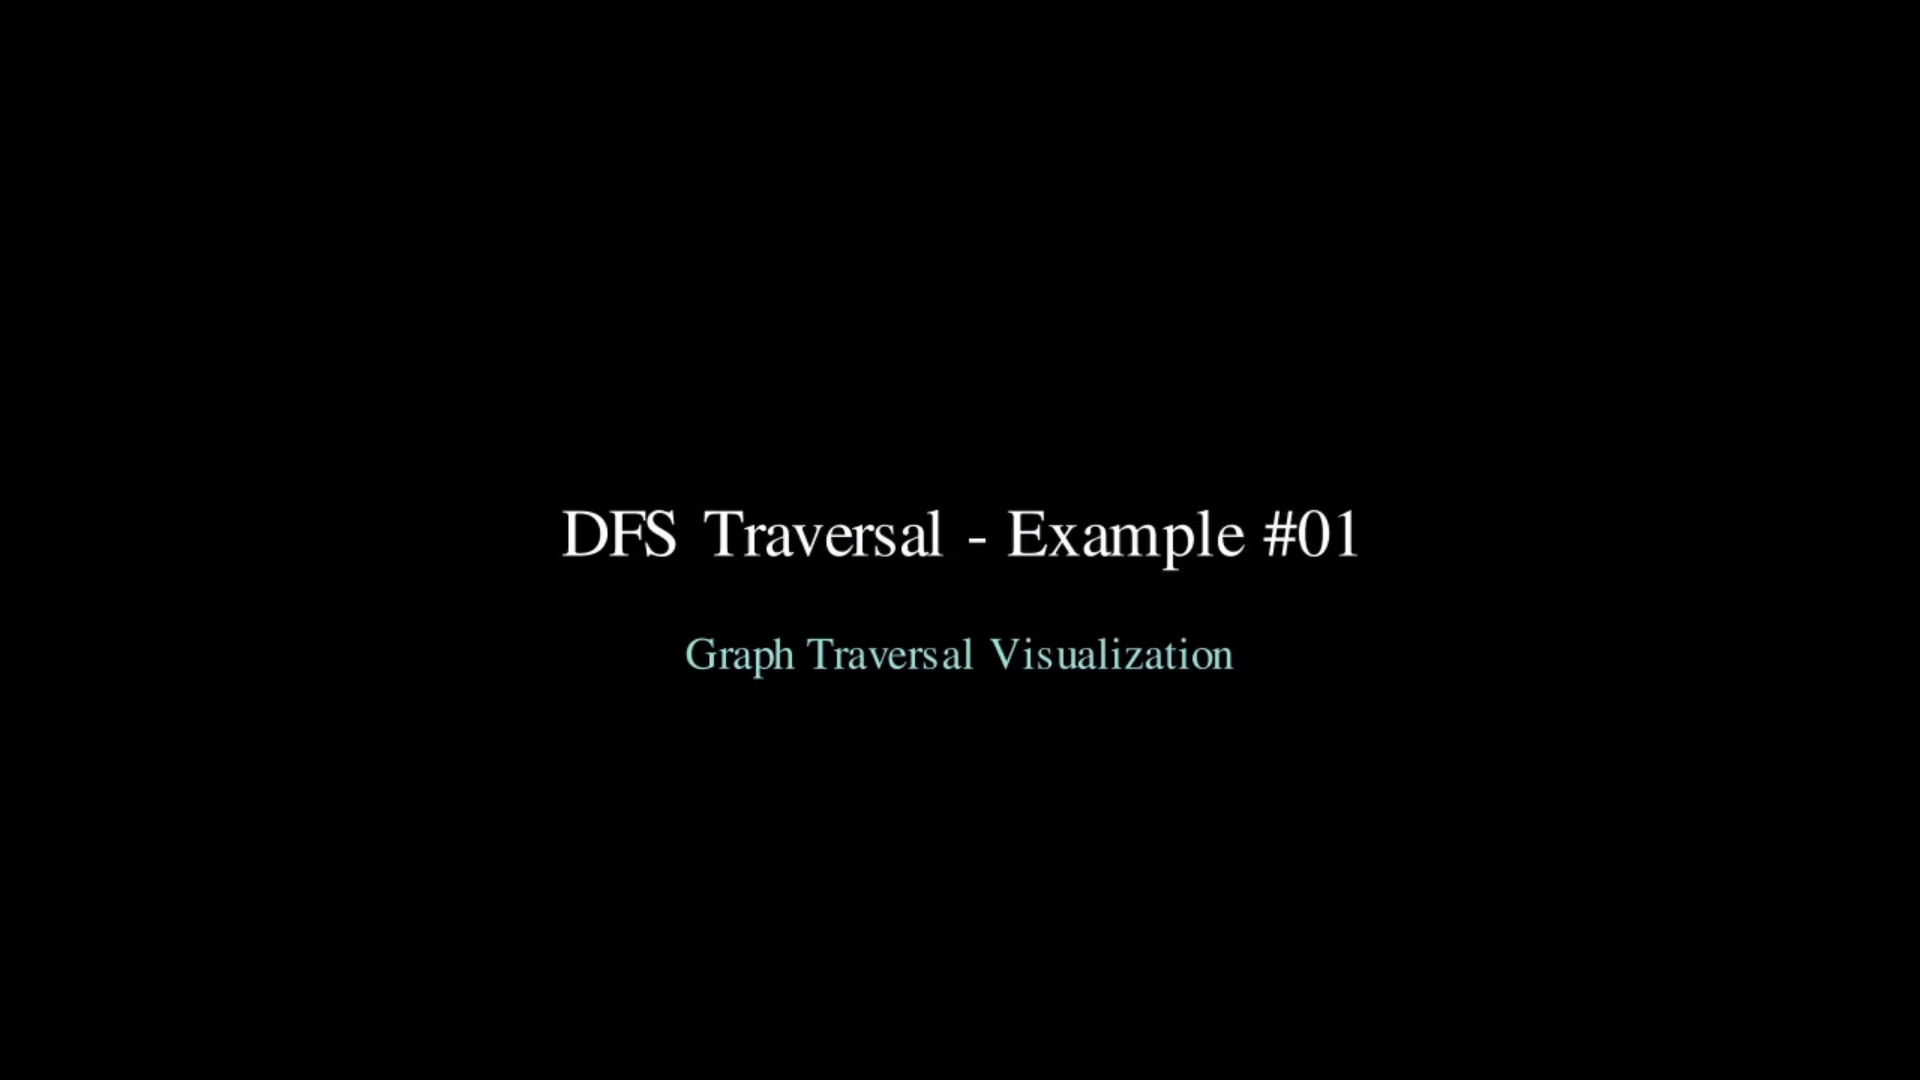
\includegraphics[width=\linewidth]{figures/general/dfs.png}}
    \end{center}
\end{frame}

\begin{frame}
    \frametitle{Example \# 02}
    \begin{center}
        \href{https://drive.google.com/file/d/1XyJkYkLB1R2ga_u92-TW8_92aolGSF1Q/view?usp=sharing}{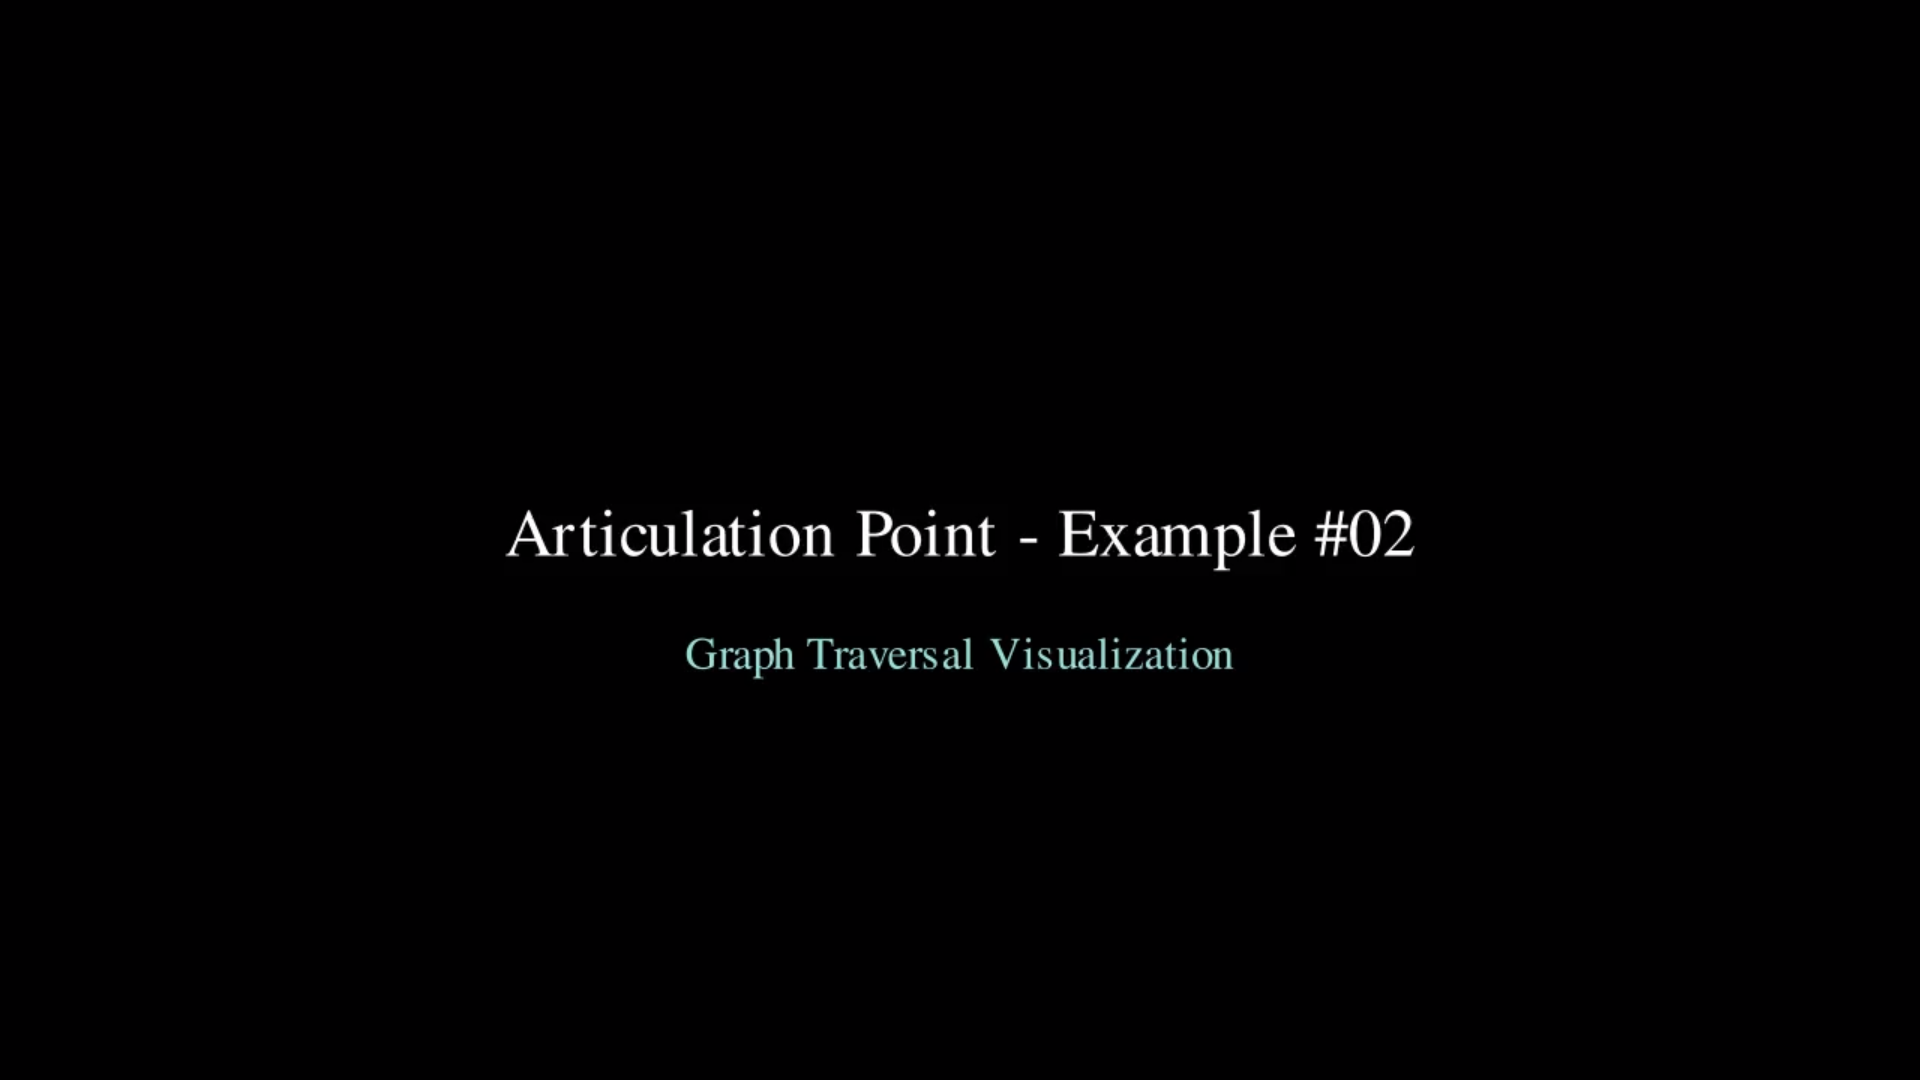
\includegraphics[width=\linewidth]{figures/general/exm02.png}}
    \end{center}
\end{frame}

\begin{frame}
    \frametitle{Example \# 03}
    \begin{center}
        \href{https://drive.google.com/file/d/1Pkawh6ed-hFe0QVqyvusOChsjhh7yxKG/view?usp=sharing}{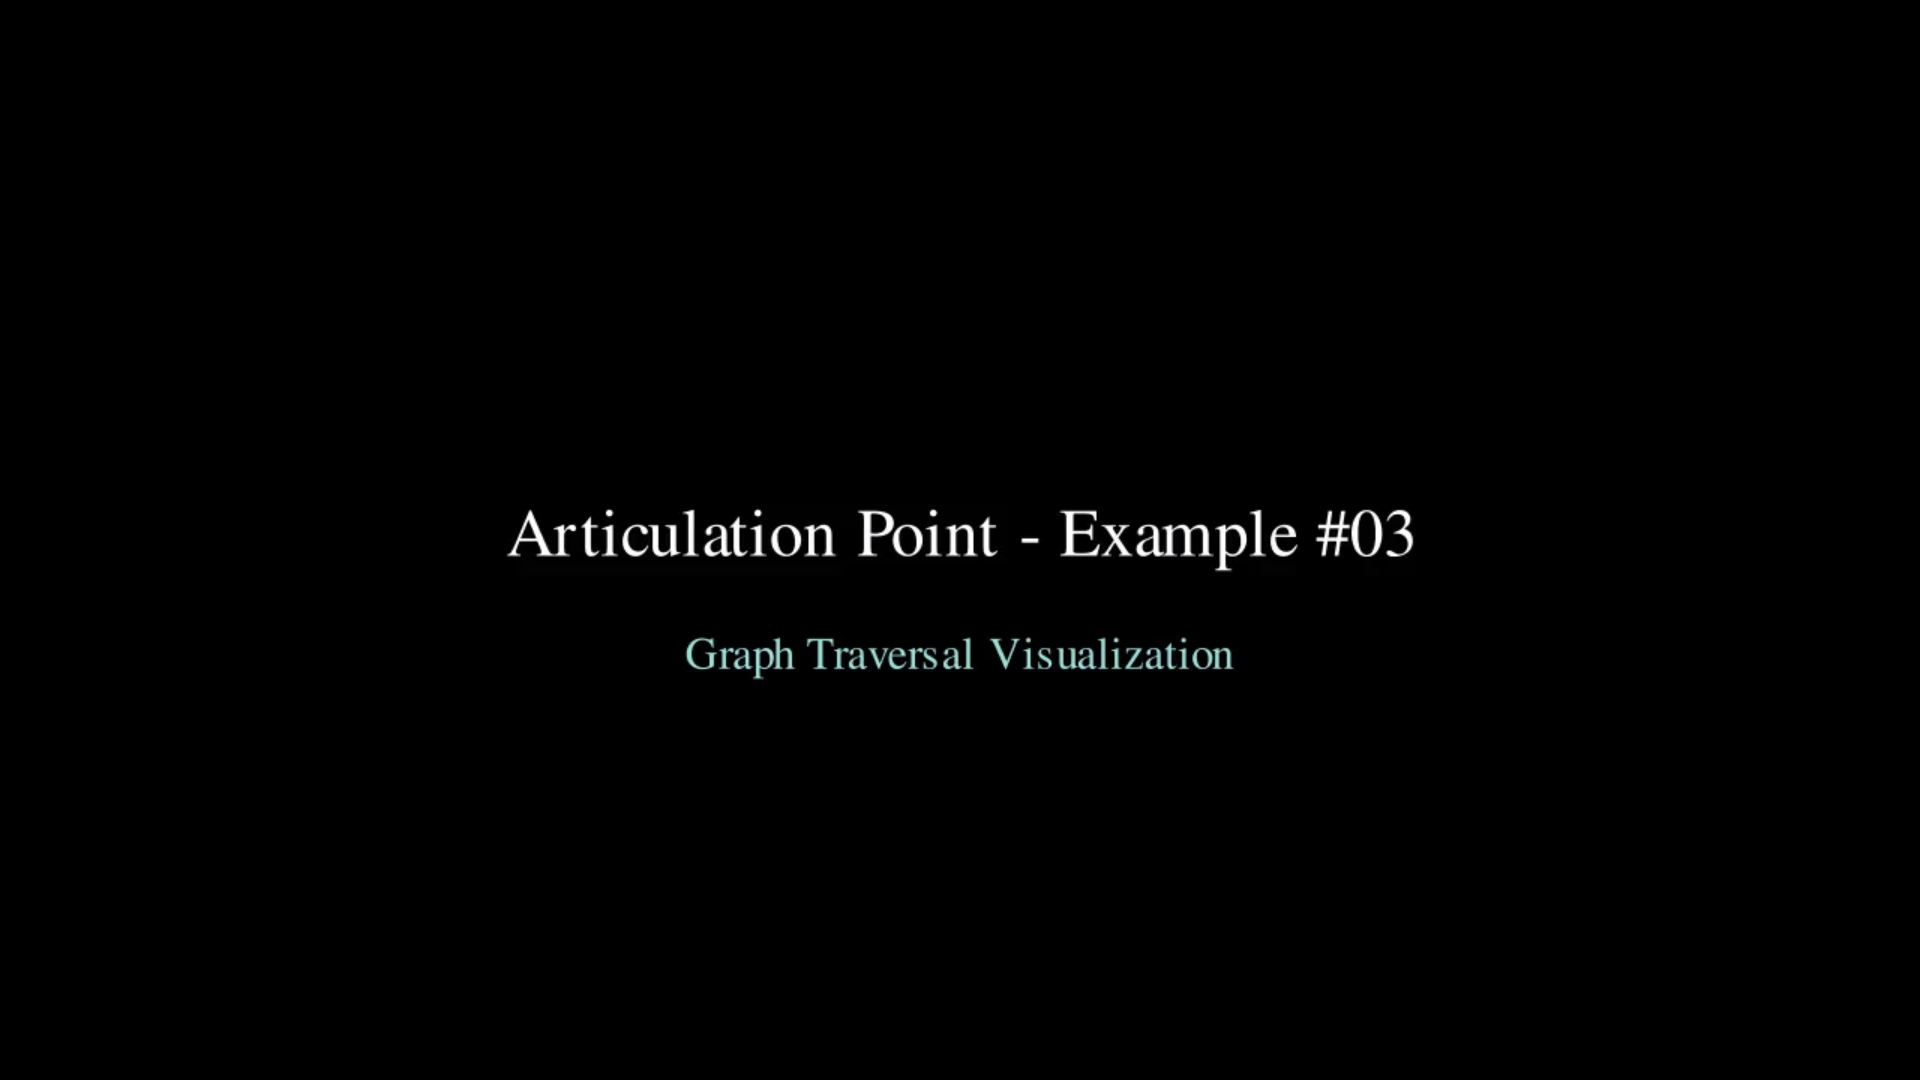
\includegraphics[width=\linewidth]{figures/general/exm03.png}}
    \end{center}
\end{frame}

\begin{frame}
    \frametitle{Example \# 04}
    \begin{center}
        \href{https://drive.google.com/file/d/1fK3Roh2BQrmu08Y9DjCE91dDoYBKczVv/view?usp=sharing}{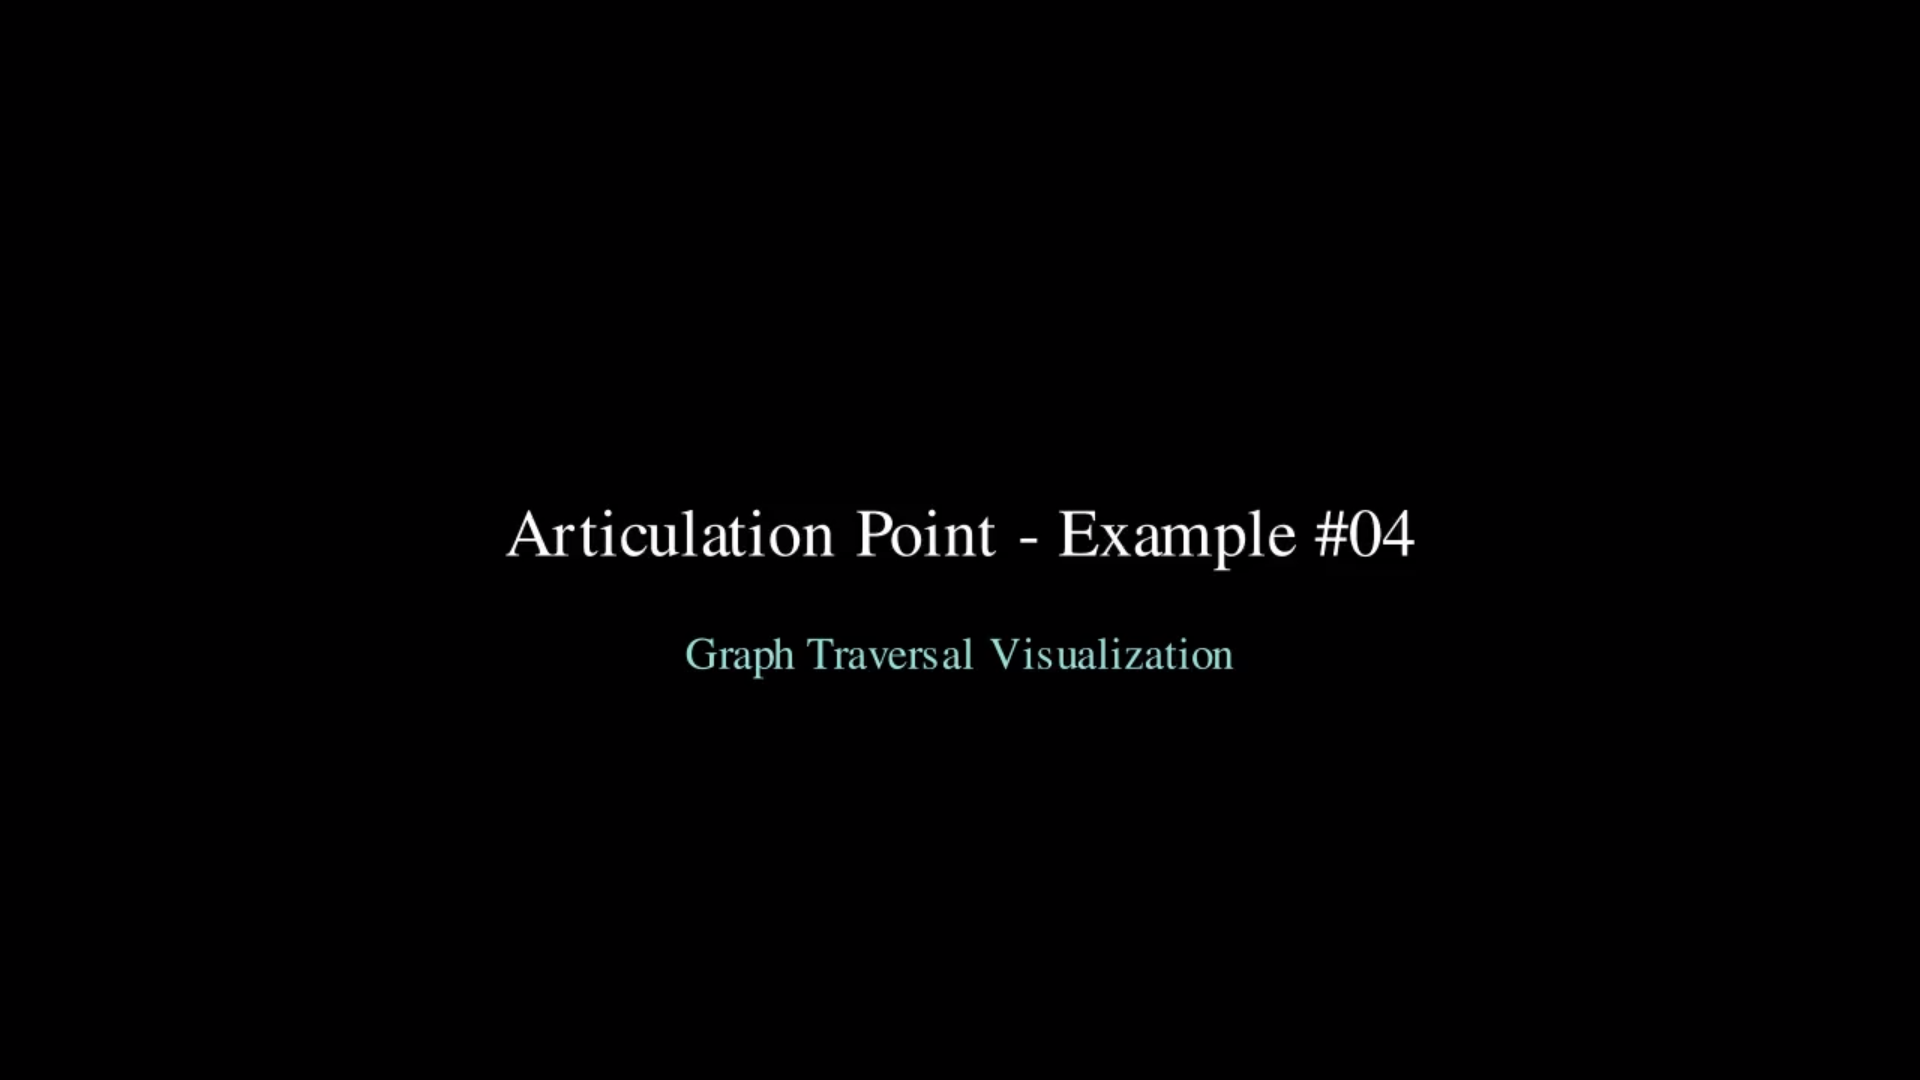
\includegraphics[width=\linewidth]{figures/general/exm04.png}}
    \end{center}
\end{frame}

\begin{frame}
    \frametitle{SCC - Strongly Connected Components}
    \vspace{5pt}
    \begin{itemize}
        \item Strongly Connected Components (SCC) are known as connected components in a undirected graph $G$.
        \item Removing articulation point(s) causes increase in the connected components of the graph $G$
    \end{itemize}
\end{frame}

\begin{frame}
    \frametitle{Algorithm Design}
        \textbf How do you define articulation point if the given graph $G$ is already disconnected? 
    \begin{itemize}
        \item It's easy to check for Directed graph $G$, but for undirected graph $G$, let's say we are 50 level down and the current node has an edge with someone 50 levels up, that;s what we are going to do in our algorithm. 
        \item There are many more directions to account for and in worst cases sometimes a vertex is discovered which connects the same path from the descendents graph to the ancestors graph, contradicting with the articulation point found and nullifying it.
    \end{itemize}
    \vspace*{5pt}
    \textbf And the way we are going to do is to keep a track of this by time. 
    \begin{itemize}
        \item for each node, we will keep track of their top-level node (ancestor) by time. 
        \item Now, designing our algorithm we will keep a specific order of the nodes discovered through a means called, Discovery time. Helping keep track of the top level node (ancestor).
    \end{itemize}
\end{frame}

\begin{frame}
    \frametitle{Algorithm - Articulation Point}

    \textbf{DFS(\( v \))}

    \vspace{10pt}
    
    \hspace{10pt} \( d(v) = 1 \), \( l(v) = 1 \), flag = \( F \)

    \vspace{10pt}

    \hspace{10pt} \textbf{for} \( \forall u \in N(v) \) \textbf{(where \( u \) is unvisited)}:
    
    \vspace{10pt}
    
    \hspace{20pt} \textbf{\textbf{}{IF}} flag == \( F \):
    
    \vspace{10pt}
    
    \hspace{30pt} flag = \( T \)
    
    \vspace{10pt}
    
    \hspace{20pt} \textbf{\textbf{}{IF}} flag == \( T \):
    
    \vspace{10pt}
    
    \hspace{30pt} \( u.\text{articulation} = T \)
\end{frame}

\begin{frame}
    \frametitle{Algorithm - Continue}

    {\fontsize{13}{16}\selectfont \textbf{WIP: To be continued next time}} % WIP message

    \vspace{10pt} % Space after the WIP message

    \textbf{DFS(\( v \))}
    
    \vspace{5pt}
    
    \hspace{10pt} \( Time = 1 \)
    
    \vspace{5pt}
    
    \hspace{10pt} \( d(v) = Time \), \( l(v) = Time \), flag = \( F \), \( Time++ \)
    
    \vspace{5pt}
    
    \hspace{10pt} \textbf{for} \( \forall u \in N(v) \) \textbf{(where \( u \) is unvisited)}:
    
    \vspace{5pt}
    
    \hspace{15pt} \textbf{\textbf{IF}} flag == \( F \):
    
    \hspace{25pt} flag = \( T \)
    
    \vspace{5pt}
    
    \hspace{15pt} \textbf{\textbf{IF}} flag == \( T \):
    
    \hspace{25pt} \( u.\text{articulation} = T \)
    
    \vspace{5pt}
    
    \hspace{10pt} \textbf{\textbf{IF}} \( d(u) < d(v) \) \textbf{AND} \( u \neq \text{parent}(v) \):
    
    \hspace{20pt} \( l(v) = \min(l(u), d(v)) \)
    
    \vspace{10pt}
    
    \textbf{Note:} \( d(v) \) = Discovery Time, \( l(v) \) = Least Discovery Time
\end{frame}
